%\documentclass[twocolumn]{amsart}
\documentclass[journal]{IEEEtran}
\usepackage[cmex10]{amsmath}
\usepackage{tikz, amssymb,listings}

\begin{document}

%\bibliographystyle{plain}
\bibliographystyle{IEEEtran}

\title{MAC address table size design}

\author{Morten~Jagd~Christensen, Ph.D.~\IEEEmembership{Senior Member,~IEEE}% <-this % stops a space

John~Doe~Smith
%\thanks{M. Christensen is with Cobham, (e-mail: morten.jagd.christensen @ cobham.com).}% <-this % stops a space
}

\markboth{Journal of \LaTeX\ Class Files,~Vol.~6, No.~1, January~2007}%
{Shell \MakeLowercase{\textit{et al.}}: Bare Demo of IEEEtran.cls for Journals}

\maketitle

\begin{abstract}
A central feature of an Ethernet switch is the size and organization of its MAC address table. The table 
is often populated by means of hashing MAC addresses and other parameters. Often manufacturers 
use the size of this table as a marketing parameter, but the size of the table is misleading when it comes to
performance.
In this article we give a brief description of Ethernet switching followed by discussions of hashing in the context of 
Ethernet switching. A statistical model for hash collisions and how they relate to performance is presented.
Finally some specific implementations of hashing functions are described and these are used 
in simulations.  In conclusion we discuss how size constraints and performance of the hashing functions 
can lead to design descisions with regards to MAC address table implementations.
\end{abstract}


\chapter{Introduction}

æøåÆØÅ

I began writing this document as a side effect of trying to understand General Relativity, which makes 
heavy use of \myindx{differential geometry}.

Here I will show some examples of 2D surfaces embedded in 3D euclidian spaces, how to create 
curves on these surfaces and how to evaulate the length of these curves. The necessary 
mathematics is introduced but the reader is assumed to be familiar with vectors, matrices and 
\myindx{differential calculus}. Several examples are given with detailed calculations.


Chapter \ref{sec:vectors} gives some basic definitions of vectors and their properties. 
We then do a quick brush up on functions of one variable in 2-dimensions in chapter \ref{sec:2dcurves}, 
how to find the areas and lengths of these curves, etc. 
Chapter \ref{sec:coordsys} describes a number of different coordinate systems in 3-dimentional 
space and how to transform from one coordinate system to another. Following this is a short 
description of maps and projections in chapter \ref{maps}.
In chapter \ref{sec:surfaces} we show how a surface can be described as a parametrization of the 
three dimentional coordinates $\vec{r}$ by two independent variables, and how curves can be 
described as the parametrization of $\vec{r}$ by one variable. In section \ref{sec:christoffel} a 
number of detailed examples of calculations based on the metric
tensor are given.
A brief description of parallel transport of vectors along curves is given in chapter \ref{sec:parallel}. 
Chapter \ref{sec:4dcurves} extends the previous ideas to higher dimensions.

\vspace{0.5cm}
\index{latex package!amsmath}
\index{latex package!graphicx}
\index{latex package!listings}
\index{latex package!amsthm}
\index{latex package!fancyhdr}
\index{latex package!pstricks}
\index{latex package!pst-3dplot}
The document is typeset with \LaTeX a lot of different packages: \emph{\myindx{amsmath}, \myindx{graphicx}, 
\myindx{listings}, \myindx{amsthm},
\myindx{fancyhdr}},...the list goes on. The figures are created by tools with varying support for 
integration with \LaTeX\ such as \textbf{gnuplot}, \TikZ\, \emph{\myindx{pstricks}} and \emph{\myindx{pst-3dplot}} packages. 
Where numerical results are required, such as difficult 
integrals, or simplification of formulae \url{\myindx{WolframAlpha.com}} has been used as 
well as Romberg integration 
routines written in C and C++. To reduce the occurence of manual errors, the software package Maxima 
was used for symbolic manipulation of algebraic expressions. Appendix \ref{sec:tools} gives details
on how to use these tools in conjunction with \LaTeX.


\begin{figure}
  \begin{center}
  \psset{unit=0.75} 
  \begin{pspicture}(-5.5,-7)(4.5,4) 
    \psset[pst-solides3d]{viewpoint=20 120 30 rtp2xyz, Decran=50,lightsrc=-10 15 10}
    \defFunction{shell}(u,v) 
        {1.2 v exp u Sin dup mul v   Cos mul mul} 
        {1.2 v exp u Sin dup mul v   Sin mul mul} 
        {1.2 v exp u Sin u   Cos mul mul}
    \psSolid[object=surfaceparametree, linecolor=black!70, base=0 pi pi 4 div neg 5 pi mul 2 div, 
         hue=0 1, fillcolor=blue!50,incolor=black!90, function=shell,linewidth=0.5\pslinewidth,ngrid =40]% 
  \end{pspicture}
\end{center}
\vspace{1cm}
\begin{center}
Mathematical surface of a \myindx{logaritmic spiral} very similar to the one created by the \emph{\myindx{Nautilus pompilius}} cephalopod.
\end{center}
\end{figure}

\section{bins and buckets}
\IEEEPARstart{A}{} 
typical implementation of a MAC address forwarding table is 
to make an array of $W$ buckets or bins each able to hold a number
of MAC address entries. We call this number the depth $d$ of the table.

A MAC address table is often specifiied in terms of its size (in entries), but an ASIC designer is probably more concerned with 
how many gates it occupies, the latter being proportional to the number of bits. Given the switch parameters $(n,d)$ the size 
is simply $n\cdot d$. If the size (in bits) of each entry is $s$, the  number of gates are $\approx n\cdot d \cdot s$.



\begin{table}[!t]
\renewcommand{\arraystretch}{1.3}
\caption{ A MAC address table consists of a MAC address, the switch port number where the MAC address was learned
and an age field. The index is implicit but shown here to illustrate its relevance.}
\centering
\begin{tabular}{lrrr}
\hline
\bfseries mac addr. & \bfseries port & \bfseries age & \bfseries index\\ 
\hline
00:23:14:00:00:01 &  3 & 125  & 47 \\
20:00:01:01:02:03 &  17  &  50 & 1 \\
$\cdots$ & $\cdots$ & $\cdots$ & $\cdots$ \\
64:b9:e8:bc:87:1c &  4 & 85   & 47 \\
\hline
\end{tabular}

\end{table}




Mapping a MAC address to a specific bin is typically done by applying a hashing 
function, $h$,  to the $M$ bit MAC address and associated information,  into the $W$ bins.


A hash function, h,  is a surjective function from a domain $\{0,\ldots,2^{n -1}\}$ of addresses to a domain $\{0,\ldots,2^{ m-1}\}$ of indices, 
where $m < n$. Borrowing a notation from cryptography, $h$ maps a bit string of length $n$ into a bit string of length $m$.

$$
   h: \{01\}^m \rightarrow \{01\}^{n}
$$

One popular method is to divide the MAC address into 4,6,8 or 12 bit chunks and then 
XOR these together. The final value identifies the bucket in which
the MAC address should be stored. Later we will discuss some specific hashing functions.

Since the final hash value has many fewer bits than the original data, it will clearly be the case
that multiple MAC addresses will map to the same hash value. This is called a hash collision.



\section{Mac address hash collisions}

\IEEEPARstart{L}{et} us assume that the MAC address table in an Ethernet switch has the parameters $(n,d)$, where $n$ is the width of the 
address table and $d$ is the depth. Any incoming MAC address is hashed into one of $n$ slots and stored
in one of the $d$ entries. If two different MAC addresses hashes into the same slot we call it a (hash) collision.
 If the slot is already full the switch will replace the oldest entry with the new one. This means that the old value is no longer 
available for making a forwarding descision and whenever a packet arrives destined for this address, the packet
will be forwarded on all ports. So hash collisions leads to flooding.

In the following we will provide some formulae for the probability of flooding as a function of the parameters $(n,d)$ and 
the number of active mac addresses $N$ in the network.

\begin{figure}
\begin{center}
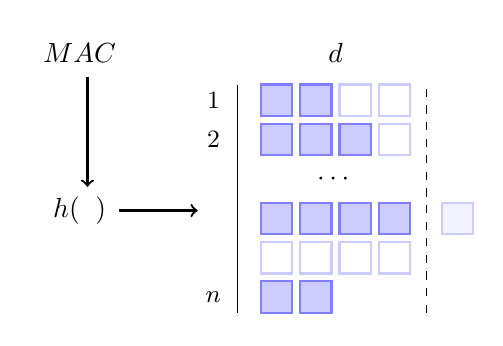
\begin{tikzpicture}
[inner sep=2mm,
box/.style={inner sep=2mm, draw=blue!50,fill=blue!20,thick},
boxe/.style={inner sep=2mm, draw=blue!20, thick},
boxf/.style={inner sep=2mm, draw=blue!20, fill=blue!5, thick}]
\draw ( 1.75 ,3.1) node {$d$};
\draw (-1.5, 3.1) node {$MAC$};
\draw (-1.5, 1.1) node {$h( \; \; )$};
\draw [->, thick] (-1.4, 2.8) to (-1.4, 1.4);
\draw [->, thick] (-1.0, 1.1) to (0.0, 1.1);

\draw (1   ,2.5)     node[box] {};
\draw (1.5,2.5)     node[box] {};
\draw (2.0,2.5)     node[boxe] {};
\draw (2.5,2.5)     node[boxe] {};

\draw (1   ,2.0)     node[box] {};
\draw (1.5,2.0)     node[box] {};
\draw (2.0,2.0)     node[box] {};
\draw (2.5,2.0)     node[boxe] {};

\draw (1.75, 1.5) node {$\cdots$};

\draw (0.2, 2.5) node {\small $1$};
\draw (0.2, 2.0) node {\small $2$};
\draw (0.2, 0.0) node {\small $n$};

\draw (1   ,1.0)     node[box] {};    \draw (1.5,1.0)     node[box] {};     \draw (2.0,1.0)     node[box] {};
\draw (2.5,1.0)     node[box] {};  \draw (3.3,1.0)     node[boxf] {};
\draw (1   ,0.5) node[boxe] {};   \draw (1.5,0.5) node[boxe] {};   \draw (2.0,0.5) node[boxe] {};   \draw (2.5,0.5) node[boxe] {};
\draw (1,   0  ) node[box] {};   \draw (1.5,0) node[box] {};

\draw (0.5,-0.2) to (0.5,2.7);
\draw [dashed] (2.9,-0.2) to (2.9,2.7);
\end{tikzpicture}
\end{center}

\caption{A model of MAC address tables in an Ethernet switch. The table parameters are
$(n,d)$ where $n$ is the number of bins and $d$, the depth,  is the number of entries in each bin.
Any MAC address is hashed into a value from $0$ to $n-1$, and if it is not already in the table it 
is added. If a bin is fully occupied, the oldest entry is discarded.}
\end{figure}


First we assume that MAC addresses are hashed into a uniform distribution. This means that any hash
value is equally probable. The actual distribution of MAC addresses is insignificant as long as the 
hashing function is sufficiently uniform. 
The probability for a MAC address to hash to slot $i$ is thus $p=1/n$. Now we will send $N$ different MAC addresses through
the switch, and
consider the probability for an arbitrary slot $i$ to contain zero, one or more entries after the experiment.
The experiment of hashing a single MAC address and observing wheter it is $i$ or not is called a Bernoulli experiment. 
Each individual Bernoulli experiment is a stochastic
variable $X$ which can have the value 1 if we hash to the value $i$, and 0 if not. 
We now repeate this Bernoulli experiment $N$ times and sums the outcomes to a new stochastic variable $Y$. 

$$
  Y = X_1 + X_2 + \cdots X_N
$$

It is easily shown \cite{Wackerly} that $Y$ is distributed according to the Binomial distribution $\mathbf{B}(N,p)$. 




$$
  Pr\{Y=y\} = \mathbf{B}(N,p) = \binom{N}{n}p^y(1-p)^{N-y}
$$
so the probability that the slot $i$ is empty (Y=0) after $N$ experiments is 
$$
   Pr\{Y=0\} = \binom{N}{0}p^0(1-p)^N = (1-p)^N
$$
if we as an example set $N=8000$ and $n=4096$ we get $(1-1/4096)^{8000} = 14.2\% $.

But how probable is it that all $d$ entries are occupied?
$$
  Pr\{Y>d\} = 1-Pr\{Y\le d\} = 1 - \sum_{y=0}^d Pr\{Y=y\}
$$

$$
  = 1- \sum_{y=0}^d \binom{N}{y} p^y (1-p)^{N-y}
$$

In our case, where $N$ is large and $p$ is small, the Binomial distribution is 
accurately approximated by the Poisson distribution with one parameter $\lambda = Np$.

$$
  Pr(Y=y) = \frac{\lambda^ye^{-\lambda}}{y!}
$$

Following the same arguments as above we get for the probability of all $d$ entries being occupied,

$$
  Pr\{Y > d\} = 1- Pr\{Y\le d \} = 1 - \sum_{y=0}^d Pr\{Y=y\}
$$

$$
 = 1 - \sum_{y=0}^d \frac{\lambda^ye^{-\lambda}}{y!}
$$

As an example of how this is useful consider the table below, where we examine the collision 
probability after exposing the switch to $N=5000$ MAC addresses. For a 16K address table with a depth
of 1 $(16K, 1)$ the probability is 3.81\%. If we keep the total size at 16K addresses but in stead
organize the table as $(8K, 2)$ the probability is now 2.41\%. If space is a limiting factor we 
could accept the 3.81\% as the target. With the parameters $(2K, 5)$ we can achieve that goal 
with only a 10K address table.

\begin{table}[h!]
\renewcommand{\arraystretch}{1.3}
\caption{Collision probability for $N=5000$ MAC addresses as function of the parameters $(n,d)$. }
\centering 
\begin{tabular}{rrrr}
\hline \hline
\bfseries n & \bfseries d & \bfseries size & \bfseries coll. prob. \\ 
\hline
16384 & 1 & 16384 & 3.81\% \\ 
8192  & 2 & 16384 &  2.41\% \\
4096  & 3 & 12288 & 3.56\% \\
2048  & 5 & 10240 & 3.82\% \\  
\hline
\end{tabular}

\end{table}

In another design situation we could state that the probability of collisions after $N=16K$ MAC addresses
should be below 0.1\% and then determine the required table size.

We now want to predict how many new MAC addresses the switch must learn before flooding happens. This is
described by the negative binomial distribution $\mathbf{NB}(r,p)$, where $r=d+1$ and $p=(1-1/n)$. Thus
if $X = \mathbf{NB}(d+1, 1-1/n)$, then
$$
   Pr\{X=x\}  = \binom{x+d}{x}(1/n)^{(d+1)}(1-1/n)^x
$$
The expectation value of $X$ is 
$$
   E(X) = \frac{pr}{1-p}
$$

It is possible to make a substantial improvement in performance by implementing 
a simple spill-over algorithm. After calculating the index $idx$ (from the hashing) we 
perform a simultaneous look up of the MAC address at addresses $idx$ and $(idx+1) \mod n$.
If there is one or more free entries , the first one is chosen. If not, we perform the usual 
operation of replacing the oldest entry by the current one.



\section{On HASH functions}
\IEEEPARstart{H}{ash}
functions are not only used for forwarding descisions, but for packet sampling \cite{Molina}, cryptography 
\cite{Sklavos2003}\cite{Kang2002} and traffic  flow analysis/prioritization \cite{Intel2009}.

 In the previous section we have assumed that 1) the distribution of 
MAC addresses is uniform or 2) that the output of the hashing algorithm
is sufficiently unpredictable. A fundamental paradigm of cryptography is that we can convert any distribution 
into a uniform distribution by means of a sufficiently effective hashing algorithm.
The various cryptographic hashfunctions MD4, MD5, SHA-1, SHA-256, etc. will certainly do the trick,
but would in this case be an overengineered solution.


but these are often too computationally intensive or introduces latency which prevents wire-speed
forwarding.
One report \cite{Stancu2003} shows that if the hashing is poorly done a MAC address size of 4096
entries can be reduced to only 80 entries effectively wasting 98\% of the address table!
In some cases, for example in the case [5], the network designer had full control over the 
distribution of MAC addresses in their network and could alleviate the problem, but this is not 
the case in general.

\subsection{XOR hashing}
The simplest hashing possible is the XOR method mentioned above. Although this method 
is far from random it is often used in practice. The main reason is
its simplicity which lends itself to parallelism, which leads to low latency implementations in ASICS.
XOR based hashing algorithms have been analyzed in \cite{Vandiren2005} and \cite{Martinez2005}.

An interesting side effect of this implementation is the good performance results it gives on standardized
test suites. In particular a switch test suite named UNH
for the institution that tests for interoperability, University of New Hampshire, mandates 
that certain tests uses linearly incrementing MAC addresses. In this case this will lead 
to an essentially perfect utilization of the MAC address table, as will be shows in the simulations.

Computing an 8 bit hash value using this method, one would simply xor together the six bytes of
the MAC address: 
$$h = MAC_1 \oplus MAC_2 \oplus MAC_3 \oplus MAC_4 \oplus MAC_5 \oplus MAC_6$$

instead of performing the xor on the 8 bit bytes, other bit-widths could be used. With some padding scheme 
essentially  any n-bit hash value up to the length (in bits) of the MAC address (and associated data)  can be 
achieved using this method.


\subsection{Pearson hashing}
Pearson hashing is a CBC-MAC using a lookup table $T$, and produces an 8 bit hash
value. Pearson hashing, or some modification of it, is used in at least one series of 
commercial switch products \cite{Intel2009}.
\lstset{language=C}
\begin{lstlisting}
  hash := 0
  for each c in C loop
    index := hash xor c
    hash := T[index]
  end loop
  return hash
\end{lstlisting}
Pearson hashing ensures that not only the individual bytes of the data stream contributes to 
the final hash value. Also their order affects the hash value. This is a necessary property 
in cryptographic systems, but not strictly needed here. Because of this property this 
algorhithm cannot be parallelized.

\subsection{Radix hashing}
Another possibility is to
consider the MAC address array as a six digit Base-R number modulus M.
If the values for R and M are chosen in a suitable manner this method 
should provide a reasonable uniform filling of the bins \cite{Sedgewick2011}. 


\lstset{language=C}
\begin{lstlisting}
  hash := 0
  R := 31
  M := 257
  for each c in C loop
    hash := (R * hash + c) mod M
  end loop
  return hash
\end{lstlisting}

There are a couple of problems with this algorithm. First the value of $M$ should be a prime number in 
order to spread the hash values  evenly, and typically a value which is a power of 2 is desired. Secondly
the method uses the modulus operation which is fairly slow.



\section{Simulations}
\IEEEPARstart{H}{ere}
we perform some simulations combining MAC address table models with the three hashing functions mentioned 
above. We adopt the nomenclature from \cite{Stancu2003}, in which the MAC addresses used in the simulations
are constructed by a combination of arbitrarily chosen but fixed values denoted $xx, yy$ and $zz$. $\alpha\alpha$
are linearly generated numbers and $\beta\beta$ and $\gamma\gamma$ are random numbers. For example using a value of
xx:yy:zz:$\alpha\alpha$:$\alpha\alpha$:$\alpha\alpha$ means that the vendor ID (the three first bytes) is fixed at some value, and the 
device ID (the last three bytes) are varied linearly starting at 00:00:00. The patterns we have chosen to simulate are

xx:yy:zz:00:$\alpha\alpha$:$\alpha\alpha$

$\beta\beta$:$\beta\beta$:$\beta\beta$:$\alpha\alpha$:$\alpha\alpha$:$\alpha\alpha$

$\beta\beta$:$\beta\beta$:$\beta\beta$:$\gamma\gamma$:$\gamma\gamma$:$\gamma\gamma$

and the random numbers are uniformly distributed.



\section{Conclusion}
\IEEEPARstart{W}{hen}
considering ,...


\section*{Acknowledgment}
\IEEEPARstart{T}{he}
authors would like to thank Professor Christian Kornerup Hansen, Eastern Washington University, for his
suggestions to the content and organization of this paper.


\bibliography{Master}



\end{document}
